\clearpage
\begingroup
\tcbset{myboxstyle/.append style={breakable=false}}
\section{Меры}

\subsection{Мера на полукольце}

\begin{definition}
    Пусть $S$ --- полукольцо подмножеств некоторого множества $X$.
    \textbf{Мерой на полукольце} $S$ называется функция
    $m\colon S\to[0;+\infty)$, удовлетворяющая условию
    \textbf{конечной аддитивности}: если
    \[
        A=\bigsqcup_{i=1}^{n}A_i,\qquad A,A_1,\ldots,A_n\in S,
    \]
    то
    \[
        m(A)=\sum_{i=1}^{n}m(A_i).
    \]
    Знак $\bigsqcup$ обозначает объединение попарно
    непересекающихся множеств.
\end{definition}

\Needspace{12\baselineskip}
\subsubsection{Свойства меры}

\begin{theorem}[Мера пустого множества]
    $m(\varnothing)=0$.
\end{theorem}

\begin{Proof}
    Из $\varnothing=\varnothing\sqcup\varnothing$ следует
    $m(\varnothing)=2m(\varnothing)$. Поскольку мера конечна,
    $m(\varnothing)=0$.
\end{Proof}

\begin{theorem}[Монотонность]
    Если $A,B\in S$ и $A\subseteq B$, то $m(A)\leq m(B)$.
\end{theorem}

\begin{Proof}
    По свойству полукольца
    \[
        B\setminus A=\bigsqcup_{j=1}^{k}C_j,\qquad C_j\in S.
    \]
    Следовательно,
    \[
        B=A\sqcup\bigsqcup_{j=1}^{k}C_j,
        \qquad m(B)=m(A)+\sum_{j=1}^{k}m(C_j)\geq m(A).
    \]
\end{Proof}

\begin{theorem}[Формула включений--исключений]
    Если $A,B,A\cup B\in S$, то
    \[
        m(A\cup B)=m(A)+m(B)-m(A\cap B).
    \]
\end{theorem}

\begin{Proof}
    Представим $B\setminus A=\bigsqcup_{j=1}^{k}C_j$, где $C_j\in S$.
    Тогда
    \[
        B=(A\cap B)\sqcup\bigsqcup_{j=1}^{k}C_j,
        \qquad A\cup B=A\sqcup\bigsqcup_{j=1}^{k}C_j.
    \]
    По конечной аддитивности
    \[
        m(B)=m(A\cap B)+\sum_{j=1}^{k}m(C_j),\qquad
        m(A\cup B)=m(A)+\sum_{j=1}^{k}m(C_j).
    \]
    Исключая сумму, получаем требуемое равенство.
\end{Proof}

\Needspace{24\baselineskip}
\subsection{Мера Лебега--Стилтьеса на промежутках}

Рассмотрим полукольцо
\[
    S=\{\varnothing,\R\}\cup\{(a;b]\colon a<b\}
      \cup\{(-\infty;b]\colon b\in\R\}
      \cup\{(a;+\infty)\colon a\in\R\}.
\]
Здесь $R(S)$ --- наименьшее кольцо, содержащее $S$,
а $\sigma(S)=\mathcal{B}(\R)$. Схема продолжения меры:
\[
    S\ \longrightarrow\ R(S)\ \longrightarrow\ \sigma(S).
\]

\begin{definition}
    Пусть $F\colon\R\to\R$ ограничена, не убывает и непрерывна справа.
    Положим
    \[
        F(-\infty)=\lim_{x\to-\infty}F(x),\qquad
        F(+\infty)=\lim_{x\to+\infty}F(x).
    \]
    \textbf{Мера Лебега--Стилтьеса на полукольце} $S$, порождённая $F$,
    задаётся равенствами
    \[
        \begin{aligned}
            m(\varnothing)&=0,\\
            m((a;b])&=F(b)-F(a),\\
            m((a;+\infty))&=F(+\infty)-F(a),\\
            m((-\infty;b])&=F(b)-F(-\infty),\\
            m(\R)&=F(+\infty)-F(-\infty).
        \end{aligned}
    \]
\end{definition}

\begin{Proof}[Неотрицательность и конечная аддитивность]
    Неотрицательность следует из монотонности $F$.
    Пусть $(a;b]=\bigsqcup_{j=1}^{k}(a_j;b_j]$.
    Упорядочим промежутки слева направо. Тогда
    \[
        a_1=a,\qquad b_k=b,\qquad b_j=a_{j+1}\quad(1\leq j<k).
    \]
    Следовательно,
    \[
        \sum_{j=1}^{k}m((a_j;b_j])
        =\sum_{j=1}^{k}\bigl(F(b_j)-F(a_j)\bigr)
        =F(b)-F(a)=m((a;b]).
    \]
    Для неограниченных промежутков вычисление аналогично,
    с использованием $F(-\infty)$ и $F(+\infty)$.
\end{Proof}

\Needspace{18\baselineskip}
\subsection{\texorpdfstring{$\sigma$}{σ}-аддитивность}

\begin{definition}
    Мера $m$, заданная на системе множеств $\mathcal{X}$,
    называется \textbf{$\sigma$-аддитивной}, если из условий
    \[
        A=\bigsqcup_{i=1}^{\infty}A_i,
        \qquad A,A_1,A_2,\ldots\in\mathcal{X}
    \]
    следует
    \[
        m(A)=\sum_{i=1}^{\infty}m(A_i).
    \]
\end{definition}

\begin{example}[Конечная аддитивность без $\sigma$-аддитивности]
    Пусть $S$ состоит из пустого множества и множеств $I\cap\Q$,
    где $I\subseteq[0;1]$ --- промежуток с концами $a,b$
    (любого типа, включая одноточечные промежутки).
    Положим
    \[
        m(I\cap\Q)=b-a,\qquad m(\varnothing)=0.
    \]
    Эта функция неотрицательна и конечно аддитивна.
    Для каждого $q\in\Q\cap[0;1]$ имеем
    \[
        \{q\}\in S,\qquad m(\{q\})=0.
    \]
    Перечислим рациональные числа отрезка:
    $\Q\cap[0;1]=\{q_1,q_2,\ldots\}$. Тогда
    \[
        \Q\cap[0;1]=\bigsqcup_{i=1}^{\infty}\{q_i\},
    \]
    однако
    \[
        m(\Q\cap[0;1])=1
        \ne\sum_{i=1}^{\infty}m(\{q_i\})=0.
    \]
    Следовательно, $m$ не является $\sigma$-аддитивной.
\end{example}

\clearpage
\subsection{Непрерывность вероятностной меры}

\begin{definition}
    $(\Omega,\mathcal{F},\Pr)$ --- вероятностная (колмогоровская)
    тройка, или вероятностное пространство.
\end{definition}

\begin{definition}[1. $\sigma$-аддитивность]
    Мера $\Pr$ называется \textbf{$\sigma$-аддитивной}, если
    для попарно непересекающихся $A_i\in\mathcal{F}$
    \[
        \Pr\left(\bigsqcup_{i=1}^{\infty}A_i\right)
        =\sum_{i=1}^{\infty}\Pr(A_i).
    \]
\end{definition}

\begin{definition}[2. Непрерывность снизу]
    Мера $\Pr$ называется \textbf{непрерывной снизу}, если
    для любой неубывающей последовательности
    $A_i\in\mathcal{F}$, $A_i\subset A_{i+1}$,
    \[
        A=\bigcup_{i=1}^{\infty}A_i
        \quad\Longrightarrow\quad
        \Pr(A)=\lim_{i\to\infty}\Pr(A_i).
    \]
\end{definition}

\begin{center}
    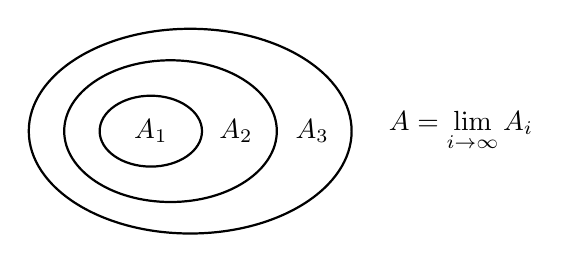
\begin{tikzpicture}
        \draw[thick] (0,0) ellipse (0.65cm and 0.45cm);
        \draw[thick] (0.25,0) ellipse (1.35cm and 0.9cm);
        \draw[thick] (0.5,0) ellipse (2.05cm and 1.3cm);
        \node at (0,0) {$A_1$};
        \node at (1.08,0) {$A_2$};
        \node at (2.05,0) {$A_3$};
        \node[right] at (2.9,0)
            {$A=\lim\limits_{i\to\infty}A_i$};
    \end{tikzpicture}
\end{center}

\begin{definition}[3. Непрерывность сверху]
    Мера $\Pr$ называется \textbf{непрерывной сверху}, если
    для любой невозрастающей последовательности
    $B_i\in\mathcal{F}$, $B_i\supset B_{i+1}$,
    \[
        B=\bigcap_{i=1}^{\infty}B_i
        \quad\Longrightarrow\quad
        \Pr(B)=\lim_{i\to\infty}\Pr(B_i).
    \]
\end{definition}

\begin{theorem}
    Для вероятностной меры на $\sigma$-алгебре условия
    1, 2 и 3 эквивалентны:
    \[
        \text{$\sigma$-аддитивность}
        \quad\Longleftrightarrow\quad
        \text{непрерывность снизу}
        \quad\Longleftrightarrow\quad
        \text{непрерывность сверху}.
    \]
\end{theorem}

\begin{Proof}[$1\implies3$]
    Пусть $B_i\supset B_{i+1}$. Положим
    \[
        A_i=B_i\setminus B_{i+1},
        \qquad B=\bigcap_{i=1}^{\infty}B_i.
    \]
    \begin{center}
        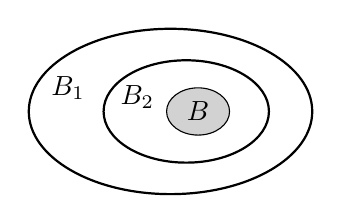
\begin{tikzpicture}
            \draw[thick] (0,0) ellipse (1.8cm and 1.05cm);
            \draw[thick] (0.2,0) ellipse (1.05cm and 0.65cm);
            \fill[gray!35] (0.35,0) ellipse (0.4cm and 0.3cm);
            \draw (0.35,0) ellipse (0.4cm and 0.3cm);
            \node at (-1.3,0.3) {$B_1$};
            \node at (-0.42,0.18) {$B_2$};
            \node at (0.35,0) {$B$};
        \end{tikzpicture}
    \end{center}
    Имеем
    \[
        \left(\bigsqcup_{i=1}^{\infty}A_i\right)\sqcup B=B_1.
    \]
    По $\sigma$-аддитивности
    \[
        \sum_{i=1}^{\infty}\Pr(A_i)+\Pr(B)=\Pr(B_1),
        \qquad \Pr(A_i)=\Pr(B_i)-\Pr(B_{i+1}).
    \]
    Следовательно,
    \[
        \lim_{n\to\infty}
        \underbrace{\sum_{i=1}^{n}
        \bigl(\Pr(B_i)-\Pr(B_{i+1})\bigr)}
        _{\Pr(B_1)-\Pr(B_{n+1})}
        +\Pr(B)=\Pr(B_1).
    \]
    Значит,
    \[
        \Pr(B_1)-\lim_{n\to\infty}\Pr(B_{n+1})
        +\Pr(B)=\Pr(B_1),
    \]
    откуда $\Pr(B)=\lim_{n\to\infty}\Pr(B_{n+1})$.
\end{Proof}


\Needspace{22\baselineskip}
\subsection{Продолжение меры с полукольца на кольцо}

Пусть $m\colon S\to[0;+\infty)$ --- мера на полукольце $S$.
Кольцо $R(S)$ состоит из конечных попарно непересекающихся
объединений элементов $S$:
\[
    R(S)=\left\{\bigsqcup_{i=1}^{n}A_i\colon
        n\in\N,\ A_i\in S\right\}.
\]

\begin{theorem}
    Для $B\in R(S)$ выберем представление
    $B=\bigsqcup_{i=1}^{n}A_i$, где $A_i\in S$, и положим
    \[
        \gamma(B)=\sum_{i=1}^{n}m(A_i).
    \]
    Тогда $\gamma$ определена корректно, является мерой на $R(S)$
    и продолжает $m$:
    \[
        \gamma(B)=m(B)\qquad\forall B\in S.
    \]
\end{theorem}

\begin{Proof}[Независимость от представления]
    Пусть
    \[
        B=\bigsqcup_{i=1}^{n}A_i=\bigsqcup_{j=1}^{k}C_j,
        \qquad A_i,C_j\in S.
    \]
    Положим $D_{ij}=A_i\cap C_j\in S$. Тогда
    \[
        A_i=\bigsqcup_{j=1}^{k}D_{ij},\qquad
        C_j=\bigsqcup_{i=1}^{n}D_{ij}.
    \]
    По конечной аддитивности $m$ имеем
    \[
        \begin{aligned}
            \sum_{i=1}^{n}m(A_i)
            &=\sum_{i=1}^{n}\sum_{j=1}^{k}m(D_{ij})\\
            &=\sum_{j=1}^{k}\sum_{i=1}^{n}m(D_{ij})
              =\sum_{j=1}^{k}m(C_j).
        \end{aligned}
    \]
    Следовательно, значение $\gamma(B)$ не зависит от выбора разбиения.
\end{Proof}

\begin{Proof}[Конечная аддитивность и продолжение исходной меры]
    Неотрицательность $\gamma$ следует из неотрицательности $m$.
    Пусть
    \[
        B=\bigsqcup_{k=1}^{r}B_k,\qquad B_k\in R(S).
    \]
    Представим каждое $B_k$ в виде
    \[
        B_k=\bigsqcup_{j=1}^{n_k}E_{kj},\qquad E_{kj}\in S.
    \]
    Все множества $E_{kj}$ попарно не пересекаются, поэтому
    \[
        \gamma(B)=\sum_{k=1}^{r}\sum_{j=1}^{n_k}m(E_{kj})
                 =\sum_{k=1}^{r}\gamma(B_k).
    \]
    Если $B\in S$, можно выбрать представление из одного множества;
    тогда $\gamma(B)=m(B)$.
\end{Proof}
\endgroup
